\documentclass[tikz,border=8pt]{standalone}
\usepackage{amsmath}
\usetikzlibrary{arrows.meta,angles,quotes}
\begin{document}
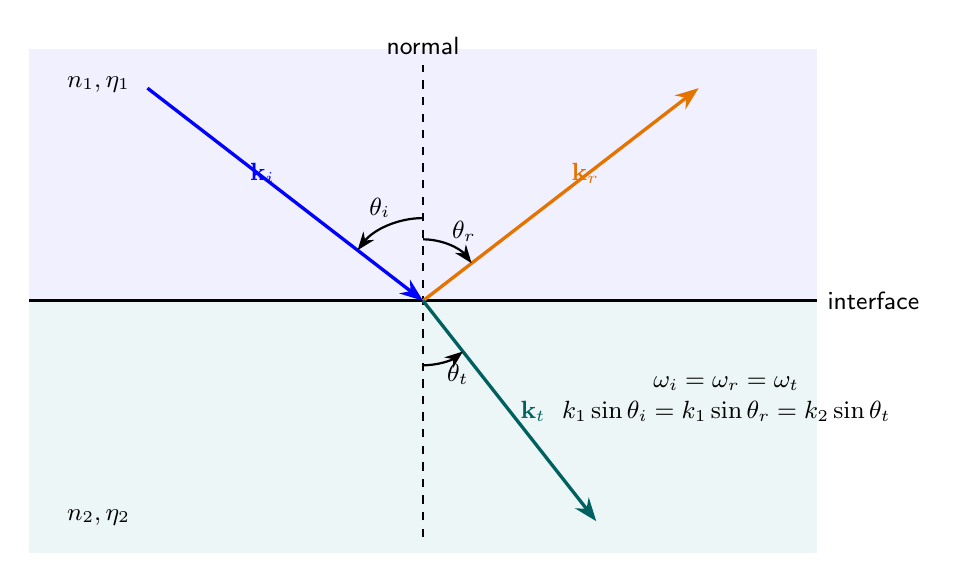
\begin{tikzpicture}[>=Stealth,font=\sffamily\small,thick]
  \fill[blue!6] (-5,0) rectangle (5,3.2);
  \fill[teal!7] (-5,-3.2) rectangle (5,0);
  \draw[very thick] (-5,0)--(5,0) node[right] {interface};
  \draw[dashed] (0,-3)--(0,3) node[above] {normal};
  \coordinate (O) at (0,0);
  \coordinate (I) at (-3.5,2.7);
  \coordinate (R) at (3.5,2.7);
  \coordinate (T) at (2.2,-2.8);
  \coordinate (N) at (0,2.2);
  \coordinate (D) at (0,-2.2);
  \draw[->,blue,very thick] (I)--(O) node[midway,above left] {$\mathbf k_i$};
  \draw[->,orange!90!black,very thick] (O)--(R) node[midway,above right] {$\mathbf k_r$};
  \draw[->,teal!75!black,very thick] (O)--(T) node[midway,right] {$\mathbf k_t$};
  \draw[->] (0,1.05) arc[start angle=90,end angle=142.3,radius=1.05];
  \node at (-.55,1.18) {$\theta_i$};
  \draw[->] (0,.78) arc[start angle=90,end angle=37.7,radius=.78];
  \node at (.52,.88) {$\theta_r$};
  \draw[->] (0,-.82) arc[start angle=-90,end angle=-51.8,radius=.82];
  \node at (.44,-.93) {$\theta_t$};
  \node[anchor=west] at (-4.65,2.75) {$n_1,\eta_1$};
  \node[anchor=west] at (-4.65,-2.75) {$n_2,\eta_2$};
  \node[align=center] at (3.85,-1.25)
    {$\omega_i=\omega_r=\omega_t$\\
     $k_1\sin\theta_i=k_1\sin\theta_r=k_2\sin\theta_t$};
\end{tikzpicture}
\end{document}
